\section{Relational convolutions with graphlet filters}\label{sec:relconv}

\subsection{Relational convolutions with discrete groups}
Suppose that we have a sequence of objects $(x_1, \ldots, x_m) \in (\mathbb{R}^{d})^m$ and a relation tensor $R \in \mathbb{R}^{m \times m \times d_r}$ describing the pairwise relations between them (obtained by a MD-IPR layer). The relational convolution operation we will define does two things: 1) extracts features of the relations between groups of objects using pairwise relations 2) transforms the relation tensor back into a sequence of objects, allowing it be composed with another relational layer to compute higher-order relations.

Fix some filter size $s < n$, where $s$ is a hyperparameter of the relational convolution layer. One `filter' is given by the \textit{graphlet} $f_1 \in \mathbb{R}^{s \times s \times d_r}$. This is a `template' for the pairwise relations between $s$ objects. Note that the dimension of the relations in this filter matches that of the input relation tensor. Let $g \subset [n]$ be a subset of the objects of size $s$. Suppose for now that $g$ is an ordered set (i.e., the group $(1, 2, 3)$ is different from the group $(2, 3, 1)$). Then, denote the relation sub-tensor given by this (ordered) subset by $R[g] := [R[i,j]]_{i,j \in g}$. We define the `relational inner product' between this relation subtensor and the filter $f_1$ by
\begin{equation}
    \label{eq:relational_inner_prod_one_filt}
    \reliprod{R[g]}{f_1} \coloneqq \sum_{i,j \in g} \iprod{R[i,j]}{f_1[i,j]}_{\reals^{d_r}} = \sum_{i,j \in g} \sum_{k \in [d_r]} R[i,j,k] f_1[i,j,k].
\end{equation}
This is simply the inner product in the corresponding euclidean space $\mathbb{R}^{s^2 d_r}$. This quantity represents how much the relations within the objects in $g$ match the relations in the template $f_1$.

% Another relevant configuration is when the relation tensor $R$ is assumed to be symmetric (i.e.: pairwise relations are symmetric). In this case, filters can be restricted to be symmetric, and can now be identified with the smaller space $\{f \in \mathbb{R}^{s \times s \times r}: f[i,j] = f[j,i] \ \forall i,j \}$. The definition of the relational inner product can be simplified in this case to $\langle R[g], f_1 \rangle_R \coloneqq \sum_{i \leq j \in g} \langle R[i,j], f_1[i,j] \rangle$.

The relational convolution layer has $n_f$ filters (a hyperparameter). Denote the collection of filters by $\boldsymbol{f} = \paren{f_1, \ldots, f_{n_f}} \in \reals^{s \times s \times d_r \times n_f}$, which we call a \textit{graphlet filter}. We define the relational inner product of a relation subtensor $R[g]$ with a graphlet filter $\bm{f}$ as the $n_f$-dimensional vector consisting of the relational inner products with each individual filter,
\begin{equation}
    \label{eq:relational_inner_prod}
    \reliprod{R[g]}{\bm{f}} \coloneq \begin{pmatrix} \reliprod{R[g]}{f_1} \\ \vdots 
 \\ \reliprod{R[g]}{f_{n_f}} \end{pmatrix} \in \mathbb{R}^{n_f}.
\end{equation}
This vector summarizes various aspects of the relations within a group, captured by several different filters\footnote{We have overloaded notation, but will use the convention that a collection of filters is denoted by a bold symbol to distinguish between the two forms of the relational inner product.}.Each filter corresponds to one dimension in the final relation-summarizing vector for the group $g$. This is reminiscent of convolutional neural networks, where each filter gives us one channel in the output tensor.

We can also define a symmetric variant of the relational inner product which is invariant to the ordering of the elements in $g$. This can be done by pooling over all permutations of $g$. In particular, we suggest max-pooling and average-pooling, although any set-aggregator would be valid. We denote the permutation-invariant relational inner product by $\iprod{R[g]}{f_1}_{\mathrm{rel}, \mathrm{sym}}$,
\begin{equation}\label{eq:symmetric_relational_inner_prod}
    \iprod{R[g]}{\bm{f}}_{\mathrm{rel}, \mathrm{sym}} \coloneq \mathrm{Pool}\paren{\set{\reliprod{R[g']}{\bm{f}} \colon g' \in g!}},
\end{equation}
\noindent where $g!$ denotes the set of permutations of the group $g$. Recall that each $\iprod{R[g']}{\bm{f}}_{\mathrm{rel}}$ is $n_f$-dimensional, and the pooling is done independently for each dimension.

For a given group $g \subset [m]$, the relational inner product with a graphlet filter, $\iprod{R[g]}{\bm{f}}_\mathrm{rel}$, gives us a vector summarizing the relational patterns inside that group. We aim to get a sequence of objects which each describes the relational patterns within each group of interest. Let $\calG$ be a set of size-$s$ groups of the the $m$ objects. The relational convolution between a relation tensor $R$ and a relational graphlet filter $\bm{f}$ is the sequence of relational inner products with each group in $\calG$,
\begin{equation}
    \label{eq:relational_convolution}
    R \ast \bm{f} \coloneq \left( \reliprod{R[g]}{\boldsymbol{f}} \right)_{g \in \calG} \equiv \left(z_1, ..., z_{\abs{\calG}}\right) \in (\mathbb{R}^{n_f})^{\abs{\calG}}
\end{equation}
$\calG$ is a pre-specified hyperparameter of the relational convolution operation. The choice depends on the usecase. If some prior information is known about reasonable groupings, this can be encoded in $\calG$. When $m$ is small and no prior information is available, a reasonable choice might be the the set of all combinations of size $s$. When $m$ is large, considering all combinations will be intractable. One solution is to consider a random sample of combinations. In the next subsections, we consider the problem of \textit{learning} the relevant groups.

% In the above, we either consider all possible groups or we somehow assume that the relevant groups $\calG$ are known and given. We may also wish to \textit{learn} the relevant groups.

\begin{figure}
    \vskip-10pt
    \centering
    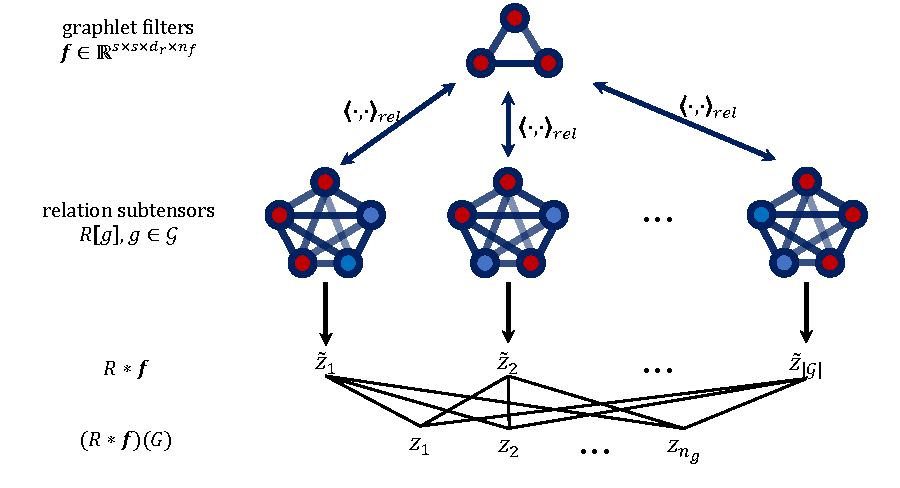
\includegraphics[width=0.9\textwidth]{figs/relconv_diagram2.pdf}
    \vskip-10pt
    \caption{A depiction of the relational convolution operation.
    % The input is a relation tensor $R$ of shape $m \times m \times d_r$, giving pairwise relations of dimension $d_r$ between a sequence of $m$ objects. A graphlet filter of size $s$ is parameterized by a relation tensor of shape $s \times s \times d_r$. The graphlet convolution operation computes relational inner products between the relation subtensor of each discrete group $g \in \calG$ with the graphlet filters $\bm{f}$. This gives a vector representation of the relations in each discrete group, $\tilde{z}_g \in \reals^{n_f}, g \in \calG$. Finally, this is synthesized into a vector representation for each of $n_g$ `soft groups', $G$, producing $(R \ast \bm{f})(G) = (z_1, \ldots, z_{n_g})$.
    }\label{fig:relconvdiagram}
    \vskip -10pt
\end{figure}

\subsection{Relational convolutions with `soft' groups}

In the above formulation, the groups are `discrete'. Having discrete groups can be desirable for interpretability, if the relevant groupings are known a priori or if considering every possible grouping is computationally and statistically feasible. However, if the relevant groupings are not known, then considering all possible combinations results in a rapid growth of the number of objects at each layer.
% Besides being computationally intractable, considering every possible grouping may be unnecessary and may make learning more difficult.

In order to address these issues, we propose \textit{explicitly modeling groups}. This allows us to control the number of objects in the output sequence of a relational convolution operation such that only relevant groups are considered. In the next section, we outline some ways to model `soft groups' using \textit{grouping layers}. These layers take a sequence of objects and/or the relation tensor as input and produce a `group matrix' $G \in \reals^{m \times n_g}$ representing $n_g$ `soft groups'. The $(i,j)$-th entry of the group matrix represents the degree to which the $i$-th object belongs to the $j$-th group. The number of groups $n_g$ is a configurable hyperparameter of the grouping layers. For the remainder of this subsection, we assume that the group matrix $G$ is given as input to the relational convolution layer.

Consider the group matrix $G \in \reals^{m \times n_g}$ and filters $\bm{f}$ of size $s$. First, we use $G$ to compute a ``group-match score'' for each discrete group $g$ of size $s$ (e.g., $g \in \calG = \binom{[m]}{s}$). This is done via
\begin{equation}\label{eq:group_match_score}
    \begin{split}
        G &\gets \text{SoftPlus}(G)\\
        \alpha_{gk} &\gets \text{Normalize}\paren{\bra{\prod_{i \in g} G[i,k]}_{g \in \calG}}, \quad g \in \calG, k \in [n_g],
    \end{split}
\end{equation}
where the soft-plus function is $\text{Softplus}(x) = \log(\exp(x + 1))$, applied elementwise. This has the effect of making the group matrix $G$ non-negative which is needed for the product of its elements to represent a ``group-match score''. The product inside the softmax is over elements in the discrete group $g \in \calG$. Hence, it will be large whenever the soft group $G_k := G[:, k]$ aligns with the discrete group $g$. $\mathrm{Normalize}(\cdot)$ normalizes the group match scores so that $\sum_{g} \alpha_{gk} = 1$. We propose the use of sparse normalizers~\citep{lahaControllableSparseAlternatives2018a} so that only a sparse subset of discrete groups in $\calG$ contribute to each soft group (see also~\Cref{ssec:computational_considerations}). In our experiments, we use `sparsemax'~\citep{martinsSoftmaxSparsemaxSparse2016}. Thus, $\alpha_{gk}$ is a normalized ``group-match score'' indicating the degree to which the discrete group $g$ matches the given soft group $G_k$.
% \footnote{Sparse normalizers would likely be appropriate alternatives to softmax here, since it would be desirable to have only a sparse subset of discrete groups in $\calG$ contribute to each soft group. Some sparse alternatives to softmax are discussed in~\citep{lahaControllableSparseAlternatives2018a}.}. %Note that the group match scores of discrete groups sum to one, $\sum_{g \in G} \alpha_{gk} = 1, \ \forall k \in [n_g]$.

Now, we can define the `soft' relational inner product \textit{given} the soft group $G_k$ by
\begin{equation}\label{eq:soft_relational_inner_prod}
    \langle R, \boldsymbol{f} \, \vert \, G_k \rangle_R \coloneqq \sum_{g \in \calG} \alpha_{gk} \iprod{R[g]}{\boldsymbol{f}}_\mathrm{rel}.
\end{equation}
This notation should be read as ``the relational inner product of the relation tensor $R$ with the graphlet filters $\boldsymbol{f}$ given the group $G_k$''. This expression is essentially a convex combination of the relational inner product with all possible discrete groups weighted by how much they match the soft group $G_k$.

With this modification, the number of objects in the output sequence is fixed and controlled by the number of groups, $n_g$ (which is a hyperparameter). The output sequence of the relational convolution given groups $G$ is now given by
\begin{equation}\label{eq:soft_relational_convolution_groups}
    (R \ast \bm{f})(G) = \left( \softreliprod{R}{\bm{f}}{G_1}, \ldots, \softreliprod{R}{\bm{f}}{G_{n_g}} \right) \in \left(\mathbb{R}^{n_f}\right)^{n_g}.
\end{equation}
